\subsection{Overview}
The following section will give an overview of the pipeline. It will explain the design decisions of the pipeline. The first section will show a step by step process of creating the pipeline, the second section will explain the various components of the pipeline and the last section will explain the technologies that were used in the pipeline.
\subsection{Steps for pipeline}
\textbf{TART}
\begin{enumerate}
    \item Load in the Data for the TART interferometer, this being, the antenna layout, the latitude and frequency and the current visibilities. Receive the cell size from the CherryPy web server.
    \item Calculate for every antenna pair, the baseline.
    \item Get the UV coordinates for the baseline and add it to the array of baselines.
    \item For each baseline add the visibilities to the array
    \item Create the grid of the size specified.
    \item Scale the UV coordinates down so that they fit onto the grid.
    \item Add the visibilities to the grid based on the position in the UV plane. Increment the counter for the grid pixel.
    \item Once all the visibilities are added, divide each cell by the counter that was created for that cell.
    \item Do the inverse FFT on the grid.
    \item Create a grid populated by 1's in the location of the UV coordinates, and do and inverse FFT on it, the point at the center of the array determines the scale factor. 
    \item Divide the image grid by the scale factor.
    \item Draw the image using imshow.
\end{enumerate}
\textbf{Testing}
\begin{enumerate}
    \item Load the custom array layout and sky model. Receive the cell size and field of view from the CherryPy web server.
    \item Calculate for every antenna pair, the baseline.
    \item Get the UV coordinates for the baseline and add it to the array of baselines. As this is over a period of time there will be an array or coordinates that creates a track.
    \item For each baseline calculate the visibilities from the sky model, this is done by using the Fourier transform. This is also over a period of time so there is an array of visibilities for each baseline.
    \item For each baseline add the visibilities array to the array
    \item Create the grid of the size specified.
    \item Scale the UV coordinates down so that they fit onto the grid.
    \item Add the visibilities to the grid based on the position in the UV plane. Increment the counter for the grid pixel.
    \item Once all the visibilities are added, divide each cell by the counter that was created for that cell.
    \item Do the inverse FFT on the grid.
    \item Create a grid populated by 1's in the location of the UV coordinates, and do and inverse FFT on it, the PSF determines the scale factor. 
    \item Divide the image grid by the scale factor.
    \item Draw the image using imshow.
\end{enumerate}
\begin{center}
    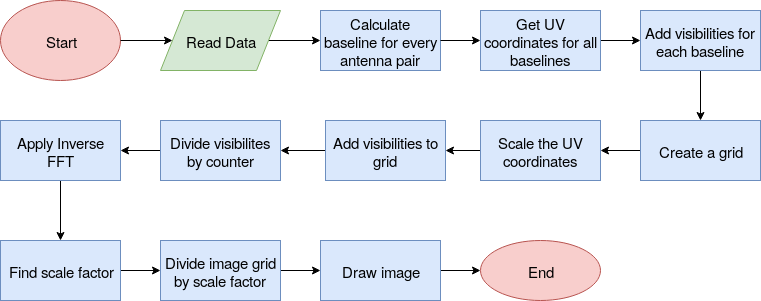
\includegraphics[scale=0.5]{images/FLOWDIAGRAM.png}
\end{center}{}
\subsection{Components}
There are three main components: Utilities, Requests and Pipeline.
\begin{center}
    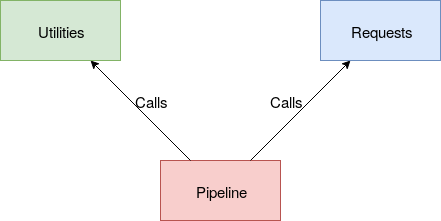
\includegraphics[scale=0.6]{images/BLOCKDIAGRAM.png}
\end{center}{}
\subsubsection{Utilities}
The utilities component contains all the functions the the imaging pipeline uses.\\
It contains all the code that plots the graphs, it contains all the code that converts from one coordinate system to another. It finds the UV tracks and the visibilities associated with them. For the custom array layout, it determines through Fourier transform the sampled visibilities of the sky model, and then plots them. It uses the cell size and field of view to create a grid of visibilities. It converts the grid of visibilities into an image.\\
The utilities are called by the pipeline component.

\subsubsection{Requests}
The requests component contains the HTTP requests for interfacing with TART, in New Zealand and South Africa, it contains three requests.
\begin{itemize}
    \item \textbf{Antenna Layout} This retrieves the the current antenna layout for the chosen TART interferometer.
    \item \textbf{Visibilities} This retrieves the latest visibilities from the chosen TART interferometer.
    \item \textbf{Latitude and Frequency} This retrieves all the information about TART, but all the pipeline needs is the latitude and frequency so the rest of the information is not used.
\end{itemize}
The requests are called by the pipeline component.

\subsubsection{Pipeline}
The pipeline is where CherryPy interfaces with python. It contains two main functions, one for the custom array layout image generation and one for the TART image generation. \\The custom layout generation takes the cell size, resolution, the baseline the user would like to see, a custom array layout of the users choosing and a sky model of the users choosing as input. It then generates the image for that sky model based off that antenna layout and sky model.\\
The TART image generation function takes the cell size, resolution and which TART interferometer the user would like to use as input. It then generates the image above the specified TART interferomter at that time.

\subsection{Technologies}
The back end is python, implementing libraries found with pip. The front end is a CherryPy web server\cite{Cherrypy} that calls the back end functions and displays the images and plots that are created. The HTML page that displays the images uses bootstrap\cite{Bootstrap} in order to display the images nicely depending on the layout of the browser.

\subsection{Usage}
Once it has been started, the tool resides on a web page at the IP address 127.0.0.1 with port 8080. On this web page there are two drop down sections, one for TART and one for custom interferometers, the latter is used for testing. Both sections require the cell size field at the top to be filled in.
\\For TART, all the user needs to do is select the TART location they wish to use and press the button labeled ``Generate new graphs", this will run the pipeline for TART and output the images onto the web page in the TART section. If the user has checked the show grid checkbox there will be a circular grid displayed on the output image for the reconstruction, If not there will be no grid. The grid that is displayed represents the relative declination from the center of the image, each circle represents an increment of 10$^\circ$ in declination, up till 90$^\circ$. 
\\In the custom interferometer section, the user needs to select a interferometer with the ``Antenna Layout" button, then select a sky model with the ``LSM file" button, the only format that the pipeline current accepts is the tigger sky model format, which uses LSM\cite{TiggerGuide}\cite{TiggerPYPI} files. The user must then select which baseline they would like to use, and what resolution they would like the output image to be, both of these are text fields. The user must then click the button labelled ``Generate Custom Graphs" and the testing pipeline will be run and an image will be produced based on the interferometer and sky model chosen. The image may also have a grid if the user has checked the checkbox.
\\The Tigger LSM format is in an HTML form with files being named as such: ``Example.lsm.html". A barebones example of the format of the file is as follows: \\
\begin{lstlisting}
<html><head>
<meta http-equiv="content-type" content="text/html; charset=windows-1252"></head>
<body mdltype="SkyModel">
<h1>Source list</h1>
<table frame="box" rules="all" cellpadding="5" border="1">
<tbody><tr mdltype="Source"><td mdltype="str" mdlval="'14_J1845M76'"><a>name:14_J1845M76</a> </td> <td mdltype="Position"><a mdltype="float" mdlval="4.9793225450667888"></a><a>ra:4.97932254507</a>  <a mdltype="float" mdlval="-1.3155380451812768"></a><a>dec:-1.31553804518</a>  </td></tr>

<h1>Other properties</h1>
<p><a mdltype="float" mdlattr="ra0" mdlval="4.9793225450667888"></a><a>Field centre ra: 4.9793225450667888</a>  <a mdltype="float" mdlattr="dec0" mdlval="-1.3155380451812768"></a><a>dec: -1.3155380451812768</a>  </p>
</body></html>
\end{lstlisting}